\documentclass[aspectratio=169]{beamer}

% Theme
\usetheme{Madrid}
\usecolortheme{seahorse}
\usefonttheme{professionalfonts}

% Packages
\usepackage{booktabs}
\usepackage{graphicx}
\usepackage{xcolor}
\usepackage{tikz}
\usepackage{pgfplots}
\pgfplotsset{compat=1.18}
\usepackage{array}
\usepackage{colortbl}
% fontawesome5 not available - using text fallbacks
\usepackage{multirow}
\usepackage{amsmath}

% Custom colors
\definecolor{mtblue}{RGB}{31,78,121}
\definecolor{mtaccent}{RGB}{70,130,180}
\definecolor{mtgold}{RGB}{212,160,23}
\definecolor{mtgreen}{RGB}{56,142,60}
\definecolor{mtred}{RGB}{198,40,40}
\definecolor{mtlightblue}{RGB}{227,242,253}
\definecolor{mtlightgray}{RGB}{245,245,245}

% Override theme colors
\setbeamercolor{frametitle}{bg=mtblue, fg=white}
\setbeamercolor{title}{fg=white}
\setbeamercolor{subtitle}{fg=mtaccent!80!white}
\setbeamercolor{author}{fg=white}
\setbeamercolor{date}{fg=white}
\setbeamercolor{institute}{fg=white}
\setbeamercolor{palette primary}{bg=mtblue, fg=white}
\setbeamercolor{palette secondary}{bg=mtaccent, fg=white}
\setbeamercolor{palette tertiary}{bg=mtblue!70, fg=white}
\setbeamercolor{block title}{bg=mtblue, fg=white}
\setbeamercolor{block body}{bg=mtlightblue}
\setbeamercolor{alerted text}{fg=mtred}
\setbeamercolor{structure}{fg=mtblue}
\setbeamercolor{itemize item}{fg=mtaccent}
\setbeamercolor{itemize subitem}{fg=mtblue!60}

% Title page styling
\setbeamertemplate{title page}{
  
\begin{tikzpicture}[remember picture, overlay]
    \fill[mtblue] (current page.north west) rectangle (current page.south east);
    \fill[mtaccent!30!mtblue] (current page.south west) rectangle +(\paperwidth, 0.08\paperheight);
    \node[anchor=north, text=white, font=\tiny] at ([yshift=-0.5cm]current page.north) {};
  \end{tikzpicture}
  \vspace{1cm}
  \begin{center}
    {\usebeamerfont{title}\color{white}\inserttitle\par}
    \vspace{0.3cm}
    {\usebeamerfont{subtitle}\color{mtaccent!80!white}\insertsubtitle\par}
    \vspace{0.5cm}
    \textcolor{white!70!mtblue}{\rule{0.6\textwidth}{0.4pt}}
    \vspace{0.4cm}
    {\color{white}\insertauthor\par}
    \vspace{0.2cm}
    {\color{white!70!mtblue}\small\insertinstitute\par}
    \vspace{0.2cm}
    {\color{white!60!mtblue}\footnotesize\insertdate\par}
  \end{center}
}

% Footer
\setbeamertemplate{footline}{
  \leavevmode
  \hbox{
    \begin{beamercolorbox}[wd=.33\paperwidth,ht=2.25ex,dp=1ex,left]{palette secondary}
      \hspace{0.5em}\footnotesize MT Benchmark: English $\rightarrow$ Hindi
    \end{beamercolorbox}
    \begin{beamercolorbox}[wd=.34\paperwidth,ht=2.25ex,dp=1ex,center]{palette tertiary}
      \footnotesize IITB Test Set
    \end{beamercolorbox}
    \begin{beamercolorbox}[wd=.33\paperwidth,ht=2.25ex,dp=1ex,right]{palette primary}
      \footnotesize\insertframenumber{}/\inserttotalframenumber\hspace{0.5em}
    \end{beamercolorbox}
  }
}

\setbeamertemplate{navigation symbols}{}
\setbeamertemplate{itemize item}{\textbullet}

% Table row colors helper
\newcommand{\rowHighlight}{\rowcolor{mtlightblue}}
\newcommand{\rowGold}{\rowcolor{mtgold!20}}

%% ============================================================
\title{Machine Translation Benchmarking}
\subtitle{Evaluating NMT Systems for English $\rightarrow$ Hindi}
\author{Benchmark Evaluation Report}
\institute{IITB Test Set $\cdot$ 4 Systems Compared}
\date{\today}
%% ============================================================

\begin{document}

%% ---- TITLE SLIDE ----
\begin{frame}[plain]
  \titlepage
\end{frame}

%% ---- OUTLINE ----
\begin{frame}{Outline}
  \tableofcontents
\end{frame}

%% ============================================================
\section{Introduction to Machine Translation}
%% ============================================================

\begin{frame}{What is Machine Translation?}
  \begin{columns}[T]
    \begin{column}{0.55\textwidth}
      \begin{block}{Definition}
        \textbf{Machine Translation (MT)} is the automated process of translating text from one natural language to another using computational models, without human intervention.
      \end{block}
      \vspace{0.3cm}
      \textbf{Key Paradigms:}
      \begin{itemize}
        \item \textbf{Rule-Based MT (RBMT)} — hand-crafted linguistic rules
        \item \textbf{Statistical MT (SMT)} — phrase/word alignment probabilities
        \item \textbf{Neural MT (NMT)} — encoder–decoder deep learning
        \item \textbf{Large Language Models} — zero/few-shot translation
      \end{itemize}
    \end{column}
    \begin{column}{0.42\textwidth}
      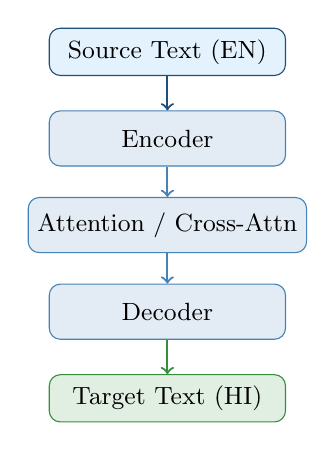
\begin{tikzpicture}[node distance=1.1cm, every node/.style={font=\small}]
        \node[draw=mtblue, fill=mtlightblue, rounded corners, minimum width=3cm, minimum height=0.6cm] (src) {Source Text (EN)};
        \node[draw=mtaccent, fill=mtaccent!15, rounded corners, minimum width=3cm, minimum height=0.7cm, below of=src] (enc) {Encoder};
        \node[draw=mtaccent, fill=mtaccent!15, rounded corners, minimum width=3cm, minimum height=0.7cm, below of=enc] (att) {Attention / Cross-Attn};
        \node[draw=mtaccent, fill=mtaccent!15, rounded corners, minimum width=3cm, minimum height=0.7cm, below of=att] (dec) {Decoder};
        \node[draw=mtgreen, fill=mtgreen!15, rounded corners, minimum width=3cm, minimum height=0.6cm, below of=dec] (tgt) {Target Text (HI)};
        \draw[->, thick, mtblue] (src) -- (enc);
        \draw[->, thick, mtaccent] (enc) -- (att);
        \draw[->, thick, mtaccent] (att) -- (dec);
        \draw[->, thick, mtgreen] (dec) -- (tgt);
      \end{tikzpicture}
    \end{column}
  \end{columns}
\end{frame}

\begin{frame}{The English–Hindi Translation Challenge}
  \begin{columns}[T]
    \begin{column}{0.48\textwidth}
      \begin{block}{Why English $\rightarrow$ Hindi?}
        \begin{itemize}
          \item Hindi has \textbf{600M+ speakers} globally
          \item Significant demand in news, government, e-commerce
          \item Morphologically rich language with complex agreement
          \item \textbf{Low-resource} relative to European language pairs
        \end{itemize}
      \end{block}
    \end{column}
    \begin{column}{0.48\textwidth}
      \begin{alertblock}{Key Linguistic Challenges}
        \begin{itemize}
          \item Script difference: Latin $\rightarrow$ Devanagari
          \item Free word order (SOV vs.\ SVO)
          \item Agglutinative morphology
          \item Named entity transliteration
          \item Code-mixing in source text
          \item Cultural / idiomatic expressions
        \end{itemize}
      \end{alertblock}
    \end{column}
  \end{columns}
  \vspace{0.3cm}
  \begin{block}{Test Set: IIT Bombay English–Hindi Corpus}
    A widely used benchmark dataset containing aligned sentence pairs sourced from diverse domains including news, government documents, and general text.
  \end{block}
\end{frame}

%% ============================================================
\section{Evaluation Metrics}
%% ============================================================

\begin{frame}{Evaluation Metrics Overview}
  \begin{columns}[T]
    \begin{column}{0.48\textwidth}
      \textbf{Lexical / N-gram Metrics}
      \vspace{0.2cm}
      \begin{itemize}
        \item \textbf{BLEU} (Bilingual Evaluation Understudy) --- precision of $n$-grams vs.\ reference; \textcolor{mtgreen}{$\uparrow$ higher is better}
        \item \textbf{chrF++} --- character $n$-gram F-score; more robust for morphology; \textcolor{mtgreen}{$\uparrow$}
        \item \textbf{TER} (Translation Edit Rate) --- edit operations to reach reference; \textcolor{mtred}{$\downarrow$ lower is better}
        \item \textbf{METEOR} --- alignment-based with synonymy; \textcolor{mtgreen}{$\uparrow$}
      \end{itemize}
    \end{column}
    \begin{column}{0.48\textwidth}
      \textbf{Neural / Semantic Metric}
      \vspace{0.2cm}
      \begin{itemize}
        \item \textbf{BERTScore-F1} --- contextual embeddings from BERT; captures semantic similarity beyond surface form; \textcolor{mtgreen}{$\uparrow$}
      \end{itemize}
      \vspace{0.4cm}
      \begin{alertblock}{Metric Limitations}
        No single metric perfectly captures translation quality. Human evaluation remains the gold standard, but automated metrics enable fast, reproducible comparison at scale.
      \end{alertblock}
    \end{column}
  \end{columns}
\end{frame}

\begin{frame}{BLEU Score in Depth}
  \begin{columns}[T]
    \begin{column}{0.55\textwidth}
      \textbf{Formula:}
      \[
        \text{BLEU} = \text{BP} \cdot \exp\!\left(\sum_{n=1}^{N} w_n \log p_n\right)
      \]
      where $p_n$ is modified $n$-gram precision and BP is the brevity penalty.
      \vspace{0.3cm}
      \begin{block}{Score Interpretation Guide}
        \begin{tabular}{ll}
          \toprule
          \textbf{BLEU Range} & \textbf{Quality Assessment} \\
          \midrule
          $<$ 10 & Poor, barely usable \\
          10 -- 19 & Hard to understand \\
          20 -- 29 & Gist conveyed \\
          30 -- 40 & Understandable \\
          40 -- 50 & Good translation \\
          50 -- 60 & High quality \\
          $>$ 60 & Near human-level \\
          \bottomrule
        \end{tabular}
      \end{block}
    \end{column}
    \begin{column}{0.42\textwidth}
      \begin{itemize}
        \item Computed over a \textbf{corpus}, not per sentence
        \item Uses \textbf{clipped} counts to avoid over-generation
        \item Correlates moderately well with human judgement
        \item \textbf{Weaknesses}: ignores synonymy, word order, morphology
        \item Especially noisy for \textbf{morphologically rich} target languages like Hindi
      \end{itemize}
      \vspace{0.3cm}
      \begin{block}{Why Multiple Metrics?}
        chrF++ and BERTScore compensate for BLEU's blind spots, especially relevant for Devanagari script output.
      \end{block}
    \end{column}
  \end{columns}
\end{frame}

%% ============================================================
\section{Systems Under Evaluation}
%% ============================================================

\begin{frame}{Systems Under Evaluation}
  \begin{columns}[T]
    \begin{column}{0.48\textwidth}
      \begin{block}{MarianMT (Helsinki-NLP)}
        \begin{itemize}
          \item Encoder–decoder Transformer
          \item Trained on OPUS parallel corpora
          \item Lightweight, fast inference
          \item Widely used baseline in research
        \end{itemize}
      \end{block}
      \vspace{0.3cm}
      \begin{block}{NLLB-600M (Meta AI)}
        \begin{itemize}
          \item No Language Left Behind initiative
          \item 200-language multilingual model
          \item 600M parameter variant
          \item Dedicated low-resource language support
        \end{itemize}
      \end{block}
    \end{column}
    \begin{column}{0.48\textwidth}
      \begin{block}{mBART-50 (Meta AI)}
        \begin{itemize}
          \item Multilingual BART pre-training
          \item Fine-tuned on 50 languages
          \item Denoising pre-training objective
          \item Strong cross-lingual transfer
        \end{itemize}
      \end{block}
      \vspace{0.3cm}
      \begin{block}{Google Translate (API)}
        \begin{itemize}
          \item Commercial neural MT system
          \item Massive proprietary training data
          \item Continuously updated model
          \item Industry gold-standard reference
        \end{itemize}
      \end{block}
    \end{column}
  \end{columns}
\end{frame}

%% ============================================================
\section{Benchmark Results}
%% ============================================================

\begin{frame}{Overall Metric Scores}
  \centering
  \renewcommand{\arraystretch}{1.4}
  \begin{tabular}{lrrrrr}
    \toprule
    \textbf{Model} & \textbf{BLEU\,$\uparrow$} & \textbf{chrF++\,$\uparrow$} & \textbf{TER\,$\downarrow$} & \textbf{METEOR\,$\uparrow$} & \textbf{BERTScore-F1\,$\uparrow$} \\
    \midrule
    MarianMT (Helsinki) & 35.50 & 30.72 & 83.15 & 28.56 & 78.92 \\
    mBART-50 (Meta)     & 48.12 & 41.53 & 77.91 & 40.60 & 83.86 \\
    NLLB-600M (Meta)    & 56.20 & 48.11 & 62.52 & 48.02 & 85.85 \\
    \rowGold
    \textbf{Google Translate} & \textbf{60.00} & \textbf{52.07} & \textbf{57.70} & \textbf{51.97} & \textbf{87.25} \\
    \bottomrule
  \end{tabular}
  \vspace{0.5cm}
  \begin{columns}
    \begin{column}{0.3\textwidth}
      \begin{block}{\centering \#1 Winner}
        \centering \textcolor{mtgold}{\large\textbullet}\\
        \textbf{Google Translate}\\
        Ranked 1st on all 5 metrics
      \end{block}
    \end{column}
    \begin{column}{0.3\textwidth}
      \begin{block}{\centering \#2 Runner-up}
        \centering \textcolor{mtaccent}{\large\textbf{2nd}}\\
        \textbf{NLLB-600M}\\
        Strong open-source choice
      \end{block}
    \end{column}
    \begin{column}{0.3\textwidth}
      \begin{alertblock}{\centering Baseline Gap}
        \centering MarianMT BLEU is\\
        \textbf{24.5 points} below\\
        Google Translate
      \end{alertblock}
    \end{column}
  \end{columns}
\end{frame}

\begin{frame}{Metrics Comparison Chart}
  \begin{center}
    
\includegraphics[width=0.85\textwidth]{mt_metrics_comparison.png}
  \end{center}
  \vspace{-0.2cm}
  \small
  \textit{Bar chart of all five metrics across the four systems. Google Translate leads on all metrics; MarianMT significantly lags. NLLB-600M is the strongest open-source system.}
\end{frame}

\begin{frame}{TER Comparison}
  \begin{center}
    
\includegraphics[width=0.82\textwidth]{mt_ter_comparison.png}
  \end{center}
  \vspace{-0.2cm}
  \small
  \textit{Translation Edit Rate (TER) — \textbf{lower is better}. Google Translate requires fewest edits (57.70) to match the reference. MarianMT requires the most edits (83.15), indicating lower fluency.}
\end{frame}

\begin{frame}{Radar Chart — Multi-Metric Profile}
  \begin{center}
    
\includegraphics[width=0.72\textwidth]{mt_radar_chart.png}
  \end{center}
  \vspace{-0.2cm}
  \small
  \textit{Radar chart showing relative normalised performance across all five metrics. Google Translate occupies the outermost position consistently; NLLB-600M is the closest open-source competitor.}
\end{frame}

\begin{frame}{Rankings Summary}
  \begin{columns}[T]
    \begin{column}{0.55\textwidth}
      \centering
      \renewcommand{\arraystretch}{1.4}
      \begin{tabular}{lcccccr}
        \toprule
        \textbf{Model} & \textbf{B} & \textbf{C} & \textbf{T} & \textbf{M} & \textbf{BS} & \textbf{Avg} \\
        \midrule
        MarianMT     & 4 & 4 & 4 & 4 & 4 & 4.0 \\
        mBART-50     & 3 & 3 & 3 & 3 & 3 & 3.0 \\
        NLLB-600M    & 2 & 2 & 2 & 2 & 2 & 2.0 \\
        \rowGold
        \textbf{Google}   & \textbf{1} & \textbf{1} & \textbf{1} & \textbf{1} & \textbf{1} & \textbf{1.0} \\
        \bottomrule
      \end{tabular}
      \vspace{0.2cm}
      {\footnotesize B=BLEU, C=chrF++, T=TER, M=METEOR, BS=BERTScore}
    \end{column}
    \begin{column}{0.42\textwidth}
      \begin{block}{Key Observations}
        \begin{itemize}
          \item Rankings are \textbf{perfectly consistent} across all metrics — no metric disagreement
          \item Google Translate's advantage is likely due to proprietary data scale
          \item NLLB-600M beats mBART-50 by \textbf{+8 BLEU} points
          \item MarianMT is \textbf{adequate as a baseline} but not production-ready for this pair
        \end{itemize}
      \end{block}
    \end{column}
  \end{columns}
\end{frame}

%% ============================================================
\section{Sentence-Level Analysis}
%% ============================================================

\begin{frame}{BLEU Score Distribution}
  \begin{center}
    
\includegraphics[width=0.85\textwidth]{mt_bleu_distribution.png}
  \end{center}
  \vspace{-0.2cm}
  \small
  \textit{Per-sentence BLEU score distributions. All models show right-skewed distributions with a long tail of low-scoring sentences, reflecting the inherent difficulty of certain sentence types.}
\end{frame}

\begin{frame}{Sentence Length vs.\ BLEU Score}
  \begin{center}
    
\includegraphics[width=0.85\textwidth]{mt_length_vs_bleu.png}
  \end{center}
  \vspace{-0.2cm}
  \small
  \textit{BLEU score as a function of source sentence length. Short sentences (1--5 tokens) generally yield higher BLEU, while longer sentences (21+ tokens) trend lower due to compounding translation errors.}
\end{frame}

\begin{frame}{Hardest \& Easiest Sentences}
  \begin{columns}[T]
    \begin{column}{0.5\textwidth}
      \textbf{\textcolor{mtred}{5 Hardest Sentences (avg BLEU)}}
      \vspace{0.15cm}
      \begin{itemize}
        \small
        \item \textit{``The water rail was fit and well by the time it was released.''} --- Idiomatic, rare vocabulary
        \item \textit{``The rep adds: `Perhaps she is confusing him...' ''} --- Quotation within quotation
        \item \textit{``Kaplowitz contends the premise that holds the most weight is the epidemic of obesity.''} --- Complex nominal structure
        \item \textit{``They never believed he died the way the sheriff concluded.''} --- Relative clause, named entity
        \item \textit{``Court blocks ruling on NYPD stop-and-frisk policy''} --- Headline, named entities
      \end{itemize}
    \end{column}
    \begin{column}{0.5\textwidth}
      \textbf{\textcolor{mtgreen}{5 Easiest Sentences (avg BLEU)}}
      \vspace{0.15cm}
      \begin{itemize}
        \small
        \item \textit{``He did not tell anyone that Jahid has drowned.''} --- Simple, high-frequency vocabulary
        \item \textit{``Today he will meet the families of the people who died in Patna last Sunday.''} --- Direct news style
        \item \textit{``A southern Georgia judge on Wednesday ordered authorities to release all surveillance video.''} --- Factual
        \item \textit{``He said: `I really want to develop an invisible ice cream.' ''} --- Simple quoted speech
        \item \textit{``They asked some subjects to count the number of dots on a computer screen.''} --- Simple active sentence
      \end{itemize}
    \end{column}
  \end{columns}
\end{frame}

%% ============================================================
\section{Error Analysis \& Conclusions}
%% ============================================================

\begin{frame}{Common Translation Error Patterns}
  \begin{columns}[T]
    \begin{column}{0.48\textwidth}
      \begin{alertblock}{MarianMT Failure Modes}
        \begin{itemize}
          \item Named entity hallucination / mistransliteration
          \item Incorrect script mixing (Latin chars in output)
          \item Dropped content words in long sentences
          \item Poor handling of numbers and dates
        \end{itemize}
      \end{alertblock}
      \vspace{0.3cm}
      \begin{block}{mBART-50 Issues}
        \begin{itemize}
          \item Occasional word-order errors
          \item Struggles with domain-specific terms
          \item Better on seen domains (news) than unseen
        \end{itemize}
      \end{block}
    \end{column}
    \begin{column}{0.48\textwidth}
      \begin{block}{NLLB-600M Strengths}
        \begin{itemize}
          \item Best open-source fluency
          \item Handles Hinglish / code-mix better
          \item Consistent across length buckets
        \end{itemize}
      \end{block}
      \vspace{0.3cm}
      \begin{block}{Sentence Length Effect}
        Across \textbf{all} models, BLEU degrades with sentence length:
        \begin{itemize}
          \item Short (1--5 tokens): avg $\sim$65+ BLEU
          \item Medium (11--20 tokens): avg $\sim$50 BLEU
          \item Long (21--35 tokens): avg $\sim$40--45 BLEU
        \end{itemize}
      \end{block}
    \end{column}
  \end{columns}
\end{frame}

\begin{frame}{Conclusions}
  \begin{columns}[T]
    \begin{column}{0.55\textwidth}
      \begin{block}{Main Findings}
        \begin{enumerate}
          \item \textbf{Google Translate} achieves the best performance across all five metrics (BLEU 60.0, BERTScore 87.25), likely due to proprietary data scale and continuous updates
          \item \textbf{NLLB-600M} is the best open-source alternative (BLEU 56.2) and viable for production use cases
          \item \textbf{mBART-50} occupies a middle ground — acceptable but beaten clearly by NLLB
          \item \textbf{MarianMT} provides a useful, lightweight research baseline but is not competitive for high-quality EN$\rightarrow$HI translation (BLEU 35.5)
          \item All models struggle with \textbf{idiomatic expressions}, \textbf{named entities}, and \textbf{long sentences}
        \end{enumerate}
      \end{block}
    \end{column}
    \begin{column}{0.42\textwidth}
      \begin{alertblock}{Recommendations}
        \begin{itemize}
          \item Use \textbf{Google Translate API} when accuracy is critical
          \item Use \textbf{NLLB-600M} for offline, privacy-sensitive, or cost-sensitive deployments
          \item Consider \textbf{domain fine-tuning} of NLLB for specialised corpora (medical, legal)
          \item Pre-process long sentences with sentence splitting to improve performance
        \end{itemize}
      \end{alertblock}
      \vspace{0.3cm}
      \begin{block}{Future Work}
        \begin{itemize}
          \item Evaluate GPT-4 / Gemini for MT
          \item Human evaluation (MQM framework)
          \item Domain-specific fine-tuning experiments
        \end{itemize}
      \end{block}
    \end{column}
  \end{columns}
\end{frame}

\begin{frame}{Summary Dashboard}
  \centering
  \renewcommand{\arraystretch}{1.6}
  \begin{tabular}{lrrrrrr}
    \toprule
    \textbf{Model} & \textbf{BLEU} & \textbf{chrF++} & \textbf{TER} & \textbf{METEOR} & \textbf{BERTScore} & \textbf{Rank} \\
    \midrule
    MarianMT      & 35.50 & 30.72 & 83.15 & 28.56 & 78.92 & \textcolor{mtred}{4\textsuperscript{th}} \\
    mBART-50      & 48.12 & 41.53 & 77.91 & 40.60 & 83.86 & \textcolor{mtblue}{3\textsuperscript{rd}} \\
    NLLB-600M     & 56.20 & 48.11 & 62.52 & 48.02 & 85.85 & \textcolor{mtaccent}{2\textsuperscript{nd}} \\
    \rowGold
    \textbf{Google Translate} & \textbf{60.00} & \textbf{52.07} & \textbf{57.70} & \textbf{51.97} & \textbf{87.25} & \textcolor{mtgreen}{\textbf{1\textsuperscript{st}}} \\
    \bottomrule
  \end{tabular}
  \vspace{0.6cm}
  
\begin{tikzpicture}
    \fill[mtgold!20, rounded corners=4pt] (0,0) rectangle (14,0.55);
    \node[font=\small, text=mtblue] at (7, 0.27) {\textbullet\textbf{Overall Winner: Google Translate} --- Best on all 5 metrics with avg rank 1.0\quad\textbullet};
  \end{tikzpicture}
\end{frame}

%% ---- THANK YOU ----
\begin{frame}[plain]
  
\begin{tikzpicture}[remember picture, overlay]
    \fill[mtblue] (current page.north west) rectangle (current page.south east);
    \fill[mtaccent!30!mtblue] (current page.south west) rectangle +(\paperwidth, 0.08\paperheight);
  \end{tikzpicture}
  \begin{center}
    \vspace{1.5cm}
    {\color{white}\Large\textbf{Thank You}}\\
    \vspace{0.5cm}
    \textcolor{mtaccent!80!white}{\rule{0.5\textwidth}{0.4pt}}\\
    \vspace{0.5cm}
    {\color{white!80!mtblue}\normalsize Machine Translation Benchmarking}\\
    \vspace{0.2cm}
    {\color{white!70!mtblue}\small English $\rightarrow$ Hindi $\cdot$ IITB Test Set $\cdot$ 4 Systems}\\
    \vspace{0.8cm}
    
\begin{tikzpicture}
      \fill[white!20!mtblue, rounded corners=4pt] (0,0) rectangle (8,0.7);
      \node[text=white, font=\small] at (4,0.35) {Data, figures, and metrics available in the accompanying repository};
    \end{tikzpicture}
  \end{center}
\end{frame}

\end{document}
